\documentclass{article}
\usepackage[utf8]{inputenc}
\usepackage{graphicx}
\usepackage{geometry}
\usepackage{algorithme}

 \geometry{
 a4paper,
 total={170mm,257mm},
 left=20mm,
 top=20mm,
 }

\title{\textbf{Projet Recherche Opérationnelle\\
Implémentation de l'algorithme de Ford Fulkerson}}
\author{BAFFERT Ambre, CASINO Lisa}
\date{10 Novembre 2020}

\begin{document}
\makeatletter
  \begin{titlepage}
  \centering
    \vspace{1cm}
      \hfill
    \vspace{1cm}
    \vfill
       {\LARGE \textbf{\@title}} \\
    \vspace{2em}
        {\large \@author} \\
    \vspace{3em}
        {\large \@date} \\
    \vfill
  \end{titlepage}
\makeatother

\newpage{}
\section{Introduction}

Au cours de l'enseignement Recherche Opérationnelle (RO), nous avons implémenté l'algorithme de Ford et Fulkerson. Nous avons utilisé l'API  GraphStream. Cet algorithme d'optimisation consiste principalement à trouver le flot maximum dans un graphe G. Nous expliquerons nos choix d'implémentations à l'aide d'une analyse descendante et de pseudo code, puis nous montrerons le résultat de notre algorithme. Nous n'avons pas géré les arc arrières dans cette version du projet.

\section{Analyse descendante}

A l'aide des cours magistraux de Mme Del Monde et du pseudo code donnée dans les PDF concernant l'algorithme général et la recherche d'une chaîne améliorante, nous avons pu concevoir l'analyse descendante ci-dessous.

\begin{figure}[!ht]
    \center
    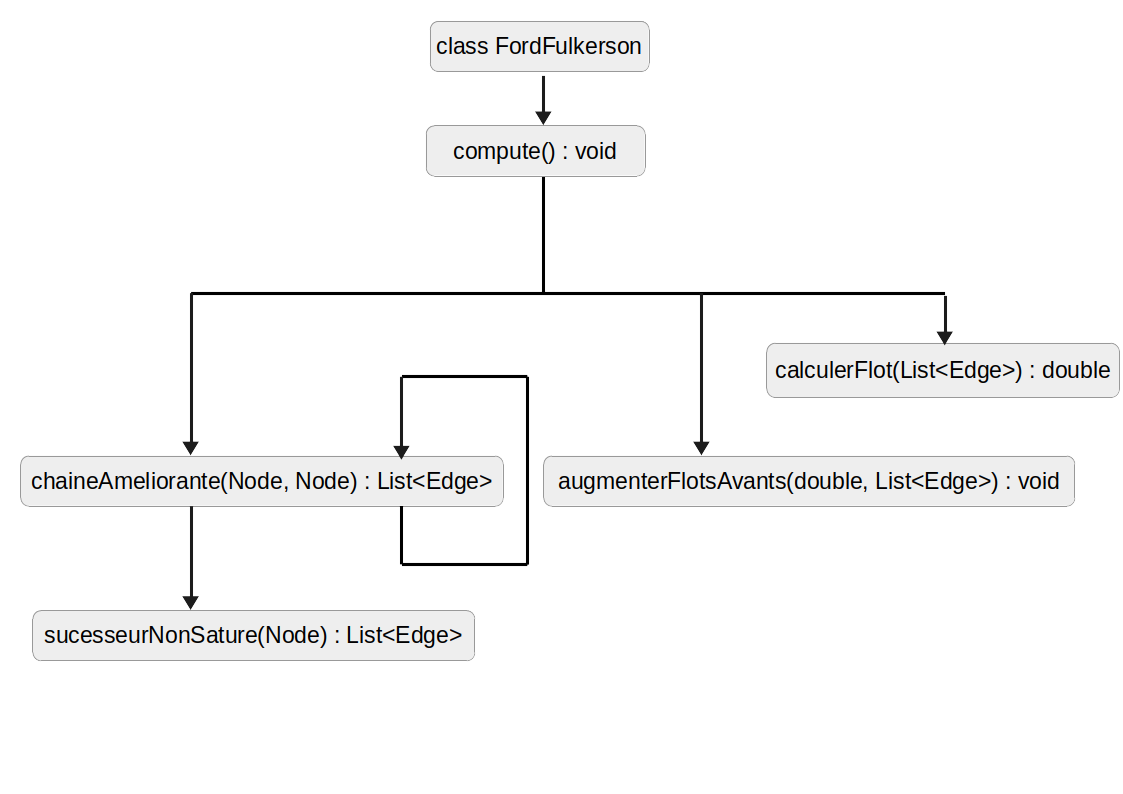
\includegraphics[width=13cm]{./images/AnalyseDescendante.png}
    \caption{Analyse descendante}
\end{figure}

Celle-ci est assez simple du fait de l'utilisation de la librairie GraphStream qui contient un grand nombre de fonctions liées à l’utilisation d’un graphe.\newline

Le fichier Flow.java récupère le fichier "graph2.dgs" qui contient les informations sur le graphe et qui se trouve dans un dossier nommé "ressource". A l'aide de la librairie graphstream et plus précisément de FlowAlgorithm, nous attribuons sur chaque arête la capacité maximale du flot et nous définissons la source et le puit. C'est ensuite que la fonction compute() est appelée. Celle-ci va chercher des chaînes améliorantes, les garder en mémoire et calculer un nouveau flot, jusqu'à ce qu'elle ne trouve plus aucune chaîne améliorante.

\section{Conception détaillée}

\subsection{compute}
\newcommand{\noeud}{\textbf{\motclefNoeud}}
\newcommand{\motclefNoeud}[0]{Noeud}
\newcommand{\arete}{\textbf{\motclefArete}}
\newcommand{\motclefArete}[0]{arete}
\begin{algorithme}
    \procedure{compute}
    {}
    {
        source,puit : \noeud ; \\
        maximumFlot : \entier ; \\
        nbAretes : \entier ; \\
        chaine : \tableauUneDimension{nbAretes}{de }{\arete} ; \\
        G : Graph ; \\ 
        Noeud1 : \noeud ; \\ 
        Noeud2 : \noeud ; \\
        delta : \reel ;

    }
    {
        \affecter{nbAretes}{getEdgeCount(G)}
        \affecter{source}{getSource(G)}
        \affecter{puit}{getSink(G)}
        \affecter{maximumFlot}{0}
        \pour{i}{0}{nbAretes}{}{
            \affecter{Noeud1}{obtenirSourceNoeud(i)}
            \affecter{Noeud2}{obtenirCibleNoeud(i)}
            \instruction{fixerFlow(Noeud1,Noeud2,0.0)}
        }
        \instruction{chargementCapacitéAttribut()}
        \instruction{affichageCapacitéArc();}
        \repeter
        {
            \affecter{chaine}{chaineAmeliorante(source,puit)}
            \sialors{estNonVide(chaine)}{
                \affecter{delta}{CalculerFlot(chaine)}
                \instruction{augmenterFlotAvant(delta,chaine)}
                \affecter{maximumFlot}{maximumFlot + delta}
            }
        }
        {estNonVide(chaine)}

    }
\end{algorithme}
\subsection{chaineAmeliorante}
\begin{algorithme}
    \fonction{chaineAmeliorante}{t,noeud : \noeud}{\tableauUneDimension{nbAretes}{de }{\arete}}
    {
        ret :\tableauUneDimension{nbAretes}{de }{\arete}
    }
    {
        \sialorssinon{noeud$=$t}
        {
            \retourner{\tableauUneDimension{0}{de }{\arete}}
        }
        {
            \pourChaque{arete}{successeurNonSature(noeud)}{

                \affecter{ret}{chaineAmeliorante(opposerDe(arete,noeud),t)}
                \sialors{estNonNul(ret)}{
                    \instruction{ajouter(ret,arete)}
                    \retourner{ret}
                }
            }
        }
        \retourner{null}
    }

\end{algorithme}
\subsection{calculerFlot}
\begin{algorithme}
    \fonction{calculerFlot} {chaine : \tableauUneDimension{nbAretes}{de }{\arete}} {\reel}
    {
        delta : \constante{MAXVALUE} \\
        temp : \reel \\
    }
    {
        \affecter{i}{0}
        \pourChaque{arete}{chaine}{
            \affecter{temp}{capacite(obtenirSourceNoeud(i),obtenirCibleNoeud(i))$-$flow(obtenirCibleNoeud(i),obtenirSourceNoeud(i))}
            \sialors{temp$<$delta}{
                \affecter{delta}{temp}
            }
        }
        \retourner{delta}
    }
\end{algorithme}

\subsection{augmenterFlotsAvants}
\begin{algorithme}
    \procedure{augmenterFlotAvants}{delta : \reel,chaine : \tableauUneDimension{nbAretes}{de }{\arete} }
    {
        Noeud1 : \noeud; \\
        Noeud2 : \noeud; \\
        newFlow : \reel; 
    }
    {
        \pourChaque{arete}{chaine}{
            \affecter{Noeud1}{obtenirSourceNoeud(arete)}
            \affecter{Noeud2}{obtenirCibleNoeud(arete)}
            \affecter{newFlow}{delta $+$ obtenirFlow(Noeud1,Noeud2)}
            \instruction{fixerFlow(Noeud1,Noeud2,newFlow)}
        }
    }
\end{algorithme}

\section{Affichage du résultat}

\subsection{Graphe}

Nous utilisons la commande "make" puis "make run" sur le terminal et avec l'aide du Makefile, le code s'exécute et voici le graphe qui est affiché dans une nouvelle fenêtre.

\begin{figure}[!ht]
    \center
    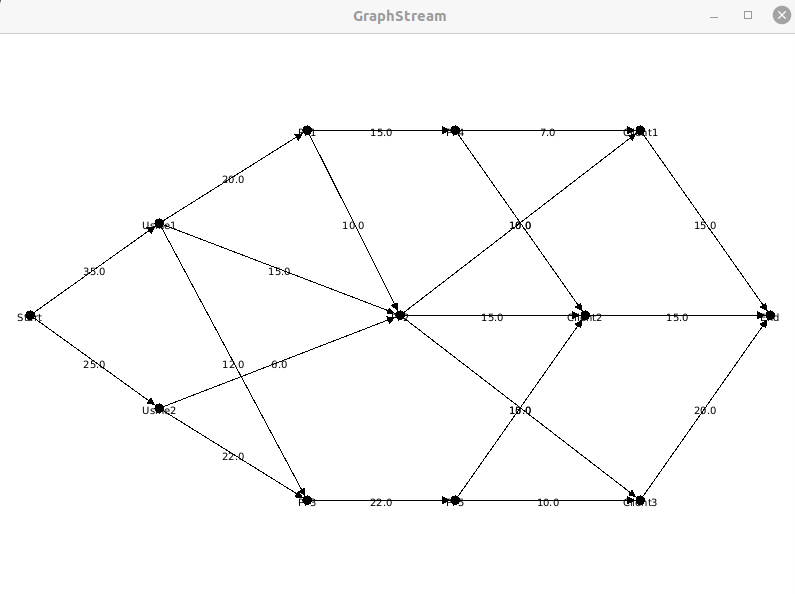
\includegraphics[width=10cm]{./images/Graphe.png}
    \caption{Affichage du Graphe}
\end{figure}

\subsection{Chaîne améliorante et flot maximal}

Après exécution du code et en même temps que le graphe s'ouvre dans une nouvelle fenêtre, les différentes chaînes améliorantes ainsi que le flot maximal que l'algorithme calcule s'affichent sur le terminal.

\begin{figure}[!ht]
    \center
    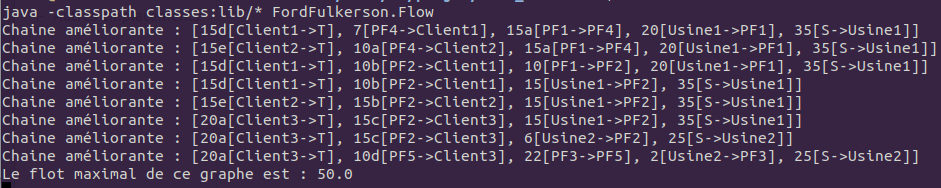
\includegraphics[width=12cm]{./images/Terminal.png}
    \caption{Résultat chaîne améliorante et flot maximal}
\end{figure}

\end{document}
